\documentclass[10pt]{article}
\usepackage{fontspec}\usepackage{luatexja-fontspec}\setmainjfont[BoldFont=FandolSong-Bold.otf,ItalicFont=FandolKai-Regular.otf]{FandolSong-Regular.otf}
\setsansjfont[BoldFont=FandolHei-Bold.otf]{FandolHei-Regular.otf}\usepackage[letterpaper,margin=.9in]{geometry}
\usepackage{amsmath,amssymb,graphicx,caption,booktabs,float,hyperref}
\captionsetup{font=small,labelfont=bf}\renewcommand{\figurename}{图}\renewcommand{\tablename}{表}
\newcommand{\Cris}{\mathcal C}\newcommand{\dd}{\,\mathrm{d}}
\newcommand{\pos}[1]{[#1]_+}\newcommand{\one}{\mathbf 1}
\title{补充数值图示：市场何时会在没有新闻的情况下崩盘？}
\author{Siyuan Ye}\date{2026 年 10 月}
\begin{document}\maketitle
\begin{center}\footnotesize 完整简体中文译本，经作者授权公开。数学内容以英文 V12 Final 原文为准。译稿日期：2026-10-15；版权保持原有声明。\end{center}
\section*{补充材料范围}
保留这些图及早期非最优两日见证，以便复现和说明。它们不是对实际市场风险的独立估计。全部数学主张和改进的区间认证构造均见主文。
\section*{早期探索性两日执行}

前述定理形成一系列层次分明的\emph{必要}检验。通过滚动区间界、标量卖出速率检验、美元闭合预处理检验及割集容量检验，仍不能证明路径存在。因此，我们从排除与下界转向\emph{同时}满足约束的构造性示例。为检验反复的\emph{部分覆盖}跌停收盘，我们构造连续的 $N=10$、$k=9$ 示例，采用 $g(S)\equiv\eta$ 市场。九项目标使用对称 $\pm3\%$ 比例区间；补偿资产采用更宽的对称 $\pm25\%$ 区间。这些是\emph{假设的归一化资产}，并非经过校准的 TSE 股票。令 $F=\eta=1$、$\rho=0.4$、相同时段长度 $\tau_1=\tau_2=20$，以及共同毛成交股数速率限制 $\bar v=1$。

记 $S_1=\cdots=S_9=x(t)$ 及 $S_{10}=y(t)$。每个时段令 $x(t)$ 为连续分段线性路径：先升至第一时段平台 $h_1$，再收于 $0.97$；随后升至第二时段平台 $h_2=0.995$，再收于 $0.97^2=0.9409$。每段斜坡持续 $0.7$ 个交易时间单位。成交金额配对通过下式唯一确定补偿资产常微分方程
\begin{equation}\label{eq:multiday-witness-ode}
 u(t)=x(t)[\dot x(t)+\rho(x(t)-1)],\qquad
 \dot y=-\rho(y-1)-\frac{9u(t)}{y(t)},\quad y(0)=1.
\end{equation}
第一平台 $h_1\approx1.0142982125$ 由\emph{精确分段多项式}方程选定
\begin{equation}\label{eq:multiday-closed}
 X_i(T_2)=\frac{x(T_2)^2-1}{2}+\rho\int_0^{T_2}x(t)[x(t)-1]\dd t=0,
 \quad i=1,\ldots,9.
\end{equation}
由于 $\dot X_{10}=-9\dot X_1$，补偿资产终端成交美元余额也闭合。独立高精度常微分方程和 Runge--Kutta 积分对 $y(T_2)$ 的结果在约 $2\times10^{-12}$ 内一致；价格区间与速率余量在密集时间网格上检查。这些数值检查是明确的\emph{见证}，并非一般 $N$ 资产充分性的证明，也不是经认证的区间包络定理。

\begin{table}[tbp]\centering\small
\caption{两个时段的 $N=10$ 确定性跌停收盘见证（归一化单位）。第 1 日与第 2 日目标损失相对重设参考价各为 $3\%$；由于补偿资产上涨，终端系统性泛函更小。}\label{tab:multiday-witness}
\begin{tabular}{@{}p{.48\linewidth}r@{}}\toprule
数量 & 已验证值 \\\midrule
九项目标收盘价，时段 1 / 时段 2 & $0.970000$ / $0.940900$\\
补偿资产收盘价，时段 1 / 时段 2 & $1.228104$ / $1.417574$\\
最大个体毛成交股数速率 & $0.680780 < \bar v=1$\\
目标成交美元余额，第 1 日 / 第 2 日 & $+0.078235$ / $-0.078235$\\
最大终端净美元余额绝对值 & $< 7\times10^{-15}$\\
配对成交金额总换手 / 最大累计卖出股数 & $2.59310$ / $1.46241$\\
终端 $\Cris_{0.9}(T_2)$ / 覆盖广度损失 $Q_{0.9}(T_2)$ & $0.019932$ / $0.060918$\\
\bottomrule\end{tabular}
\end{table}

\begin{figure}[tbp]\centering
 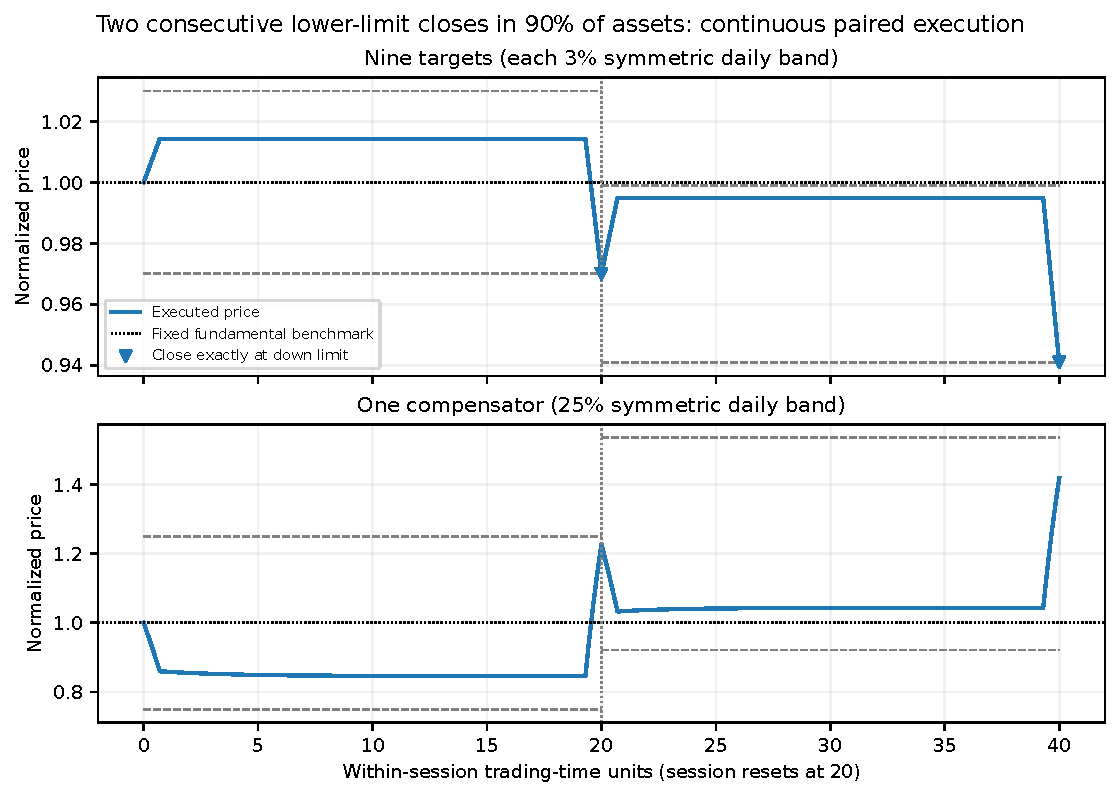
\includegraphics[width=.94\linewidth]{../../supplementary/figures/multiday_streak_witness.pdf}
\caption{\textbf{滚动每日区间下反复出现的部分覆盖跌停收盘价。} 相同九项目标资产两次收于其 3\% 下限。第十项补偿资产的区间更宽，保持在自身 25\% 限制内。图示路径没有瞬时交易。期限及区间均为规定模型输入，而非观测值。}\label{fig:streak-witness}
\end{figure}
\begin{figure}[tbp]\centering
 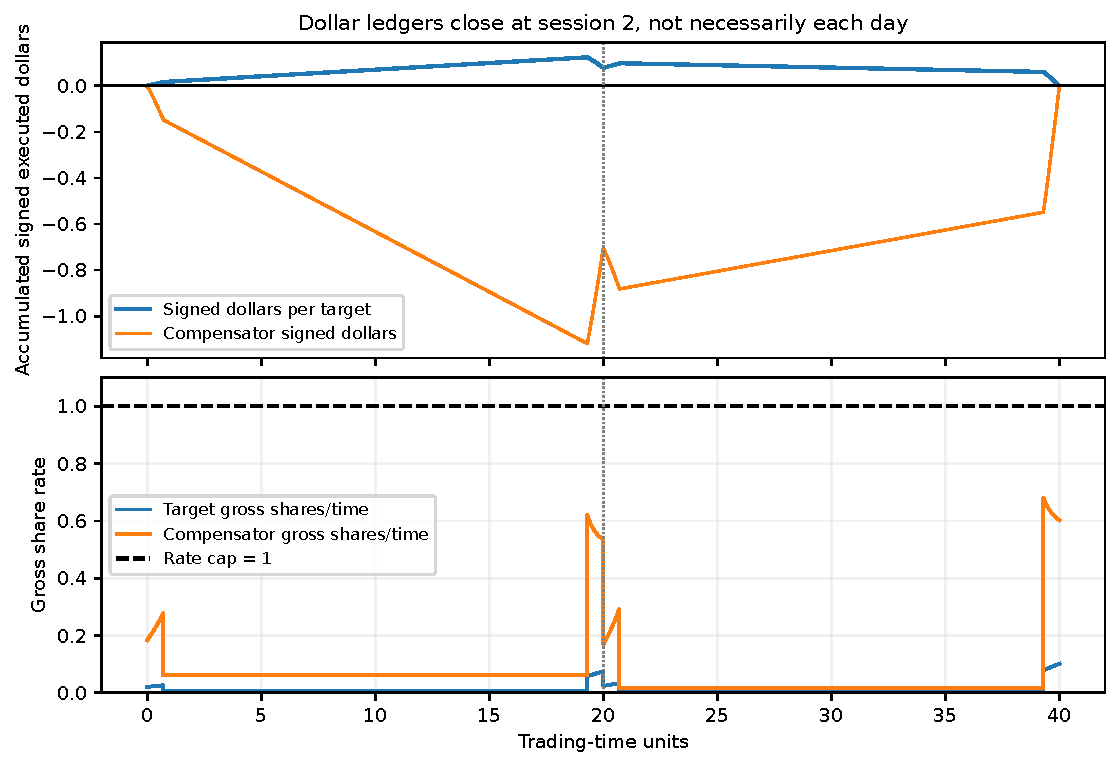
\includegraphics[width=.94\linewidth]{../../supplementary/figures/multiday_ledgers_and_rates.pdf}
\caption{\textbf{同一两时段见证的交易账簿及毛成交速率检查。} 第一时段在目标资产中积累正净美元流量；第二时段反转流量，使每项资产最终带符号美元余额为零。毛成交速率保持低于所施加股数速率限制；美元平衡连续成立，而不仅在到期时成立。}\label{fig:streak-ledger}
\end{figure}

该例既不证明交易者有动机执行该序列，也不证明存在\emph{封死}跌停订单簿。它以数值方式表明，滚动区间、有限股数成交速率、无基本面新闻冲击及终点净成交金额闭合，可以与广泛资产子集中\emph{多次}跌停收盘相容。对于危机阈值，仅有覆盖广度要求并不足够：本路径满足 $Q_{0.9}(T_2)=0.060918$，但平均损失限制起约束作用，给出 $\Cris_{0.9}(T_2)=0.019932$（因此，例如达到 $\delta=0.015$）。不能由此声称精确最小速率、最小换手或均衡发生。



\section*{其他诊断图}
\begin{figure}[tbp]
\centering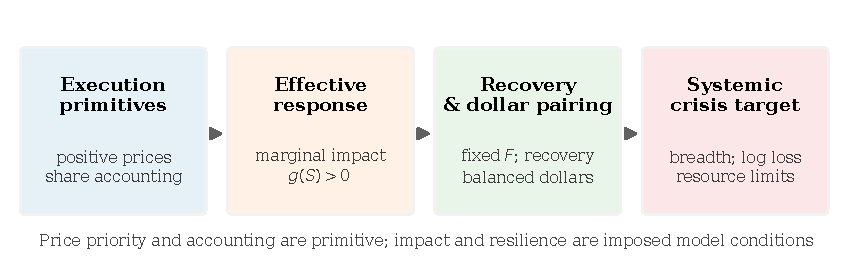
\includegraphics[width=.99\linewidth]{../../supplementary/figures/market_specification.pdf}
\caption{\textbf{一个明确定义的理想市场。} 价格优先、带符号股数核算、有效价格冲击、韧性及成交金额配对交易具有不同数学作用。本文全部定量图均为指定模型的示例，而非实时订单簿观测。}\label{fig:market}
\end{figure}
\begin{figure}[tbp]
\centering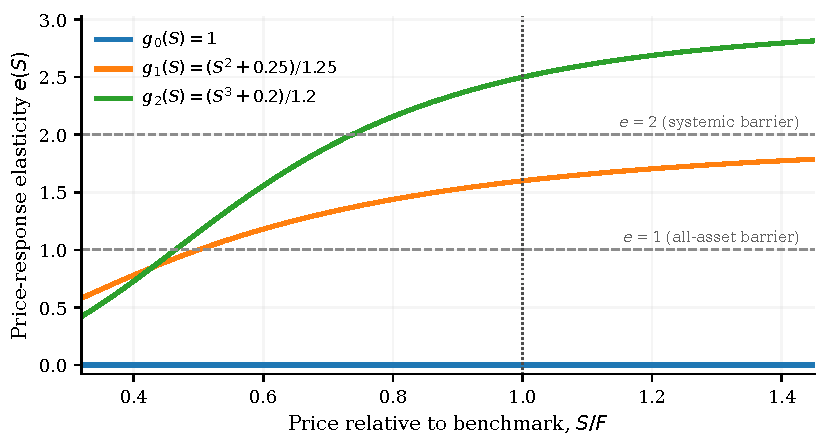
\includegraphics[width=.79\linewidth]{../../supplementary/figures/elasticity_examples.pdf}
\caption{\textbf{三个正、光滑、非幂律冲击函数的局部弹性。} 竖直虚线标记共同初始价格 $S=F$。主文的全局弹性屏障定理要求弹性不等式在整个\emph{相关可达价格区域}成立；仅有 $F$ 处的值不能给出全局分类。这是基于公式的示例，而非实证市场深度。}\label{fig:elasticity}
\end{figure}
\begin{figure}[t]
\centering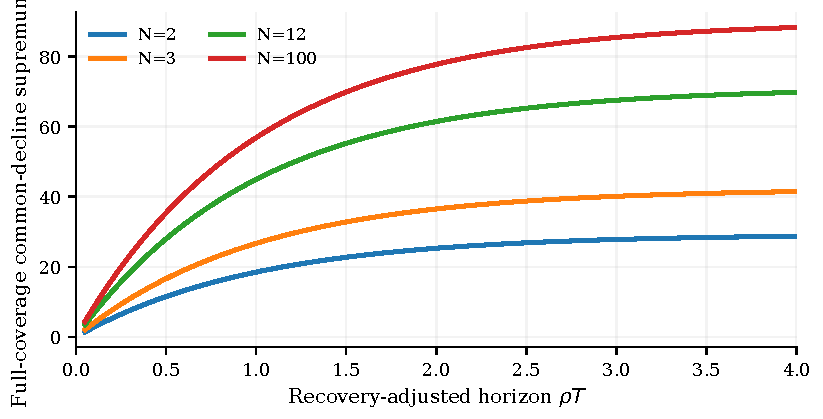
\includegraphics[width=.78\linewidth]{../../supplementary/figures/full_coverage_threshold.pdf}
\caption{\textbf{特定模型下共同下跌边界的锐界。} 对于 $g=\eta$ 及 $k=N$，共同简单价格跌幅的上包络为 $100(1-e^{-\delta_{\rm crit}})\%$。每个严格更小的对数损失阈值均能在某个有限预算下到达；严格正价格下不取到边界本身。这不是概率曲线。}\label{fig:sharp}
\end{figure}
\begin{figure}[tbp]
\centering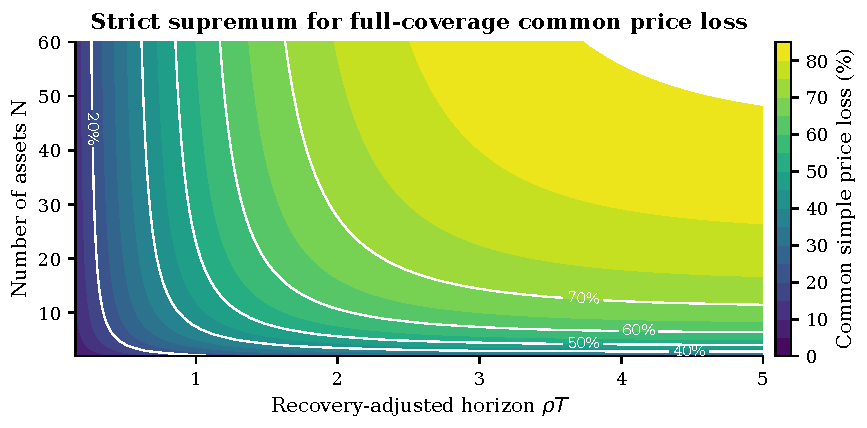
\includegraphics[width=.83\linewidth]{../../supplementary/figures/all_asset_boundary_heatmap.pdf}
\caption{\textbf{不同资产数量和恢复时间下的全覆盖边界。} 颜色表示 $100(1-e^{-\delta_{\rm crit}(N,T)})$，即恒定每股冲击及逐资产终端美元流闭合下，同时\emph{简单价格}损失的上确界。不能由此推断概率、观测回撤或有限预算最优值。}\label{fig:heatmap}
\end{figure}
\begin{figure}[tbp]
\centering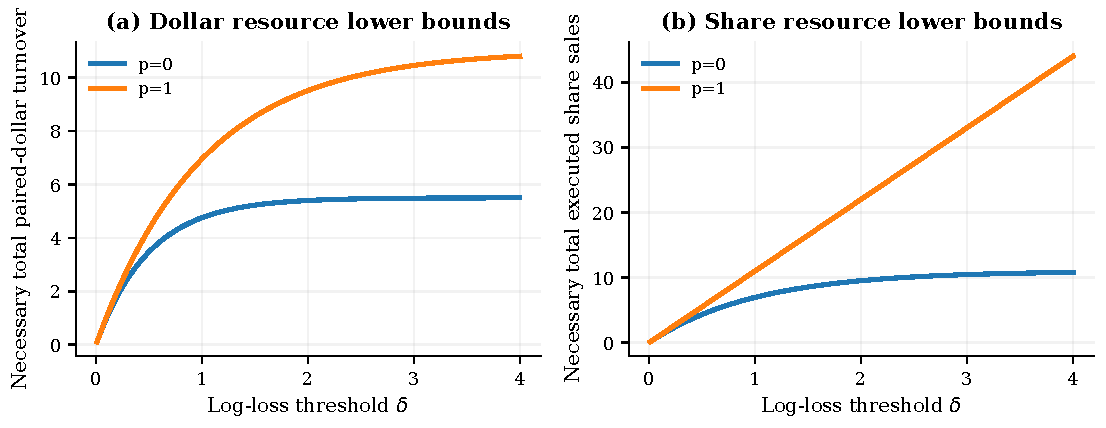
\includegraphics[width=.96\linewidth]{../../supplementary/figures/resource_lower_bounds.pdf}
\caption{\textbf{幂响应族下的一般必要资源下限示例。} 取 $F=\eta=1$、$k=11$，曲线计算 $k\int_{e^{-\delta}}^1 S/g(S)\dd S$（美元）及 $k\int_{e^{-\delta}}^1 1/g(S)\dd S$（股数），对应 $p=0,1$。这些界\emph{不是}最优执行成本，也不建立可达性。}\label{fig:resource}
\end{figure}
\begin{figure}[tbp]
\centering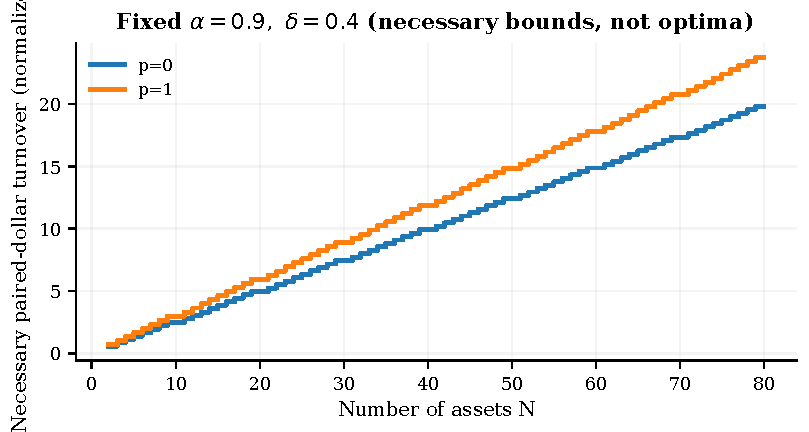
\includegraphics[width=.78\linewidth]{../../supplementary/figures/resource_scaling_N.pdf}
\caption{\textbf{必要美元资源界对资产数量的依赖。} 实验复制逐资产基准价格及响应参数，固定 $\alpha=0.9$ 与 $\delta=0.4$，并增加资产数量 $N$。台阶来自离散覆盖数量 $\lceil\alpha N\rceil$。这不是对实际股票指数按市值缩放的预测。}\label{fig:nscale}
\end{figure}
\begin{figure}[tbp]\centering
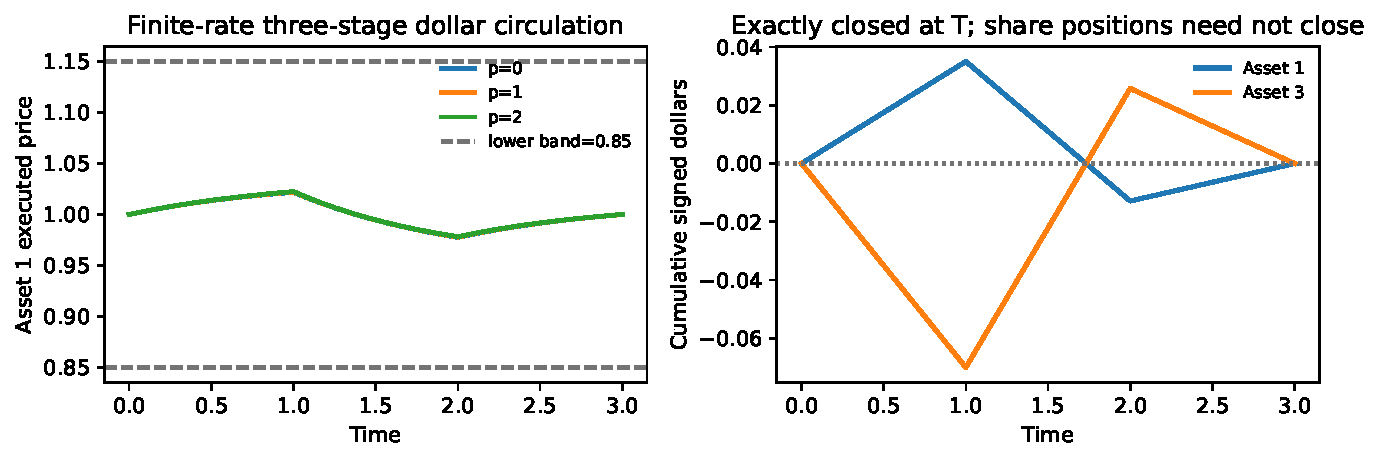
\includegraphics[width=.97\linewidth]{../../supplementary/figures/bounded_rate_continuous_path.pdf}
\caption{\textbf{新的有界速率终点净成交金额闭合路径（并非脉冲近似）。} 对于 $N=3$、$T=3$、$a=.035$、$F=\rho=\eta=1$ 及 $u=(1,1,-2)$，$p=0,1,2$ 下的价格轨迹使用相同绝对连续美元速率信号；右图展示精确闭合的美元账簿。逐资产毛成交股数速率峰值低于 $0.15$，所有价格保持在 $\pm15\%$ 区间内。}\label{fig:continuous}
\end{figure}
\begin{figure}[tbp]\centering
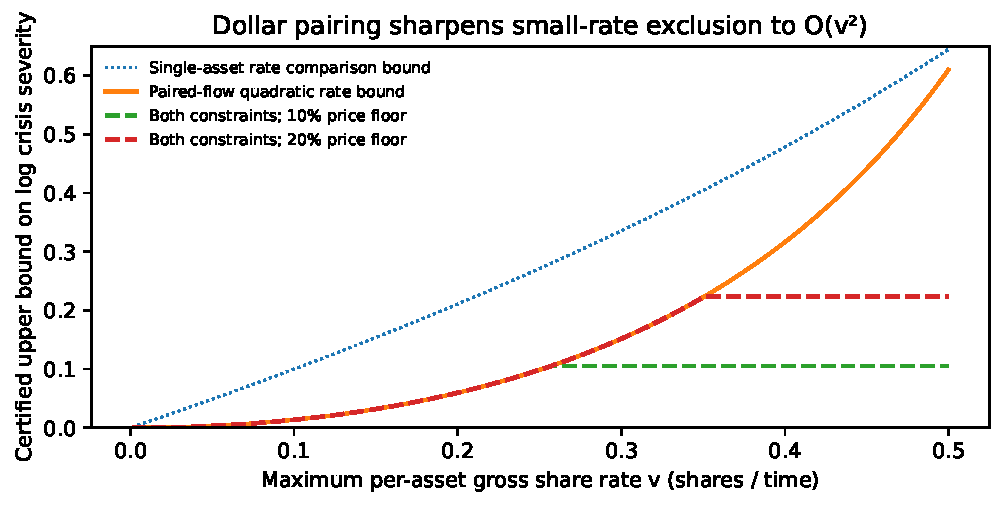
\includegraphics[width=.78\linewidth]{../../supplementary/figures/rate_and_price_limit_bounds.pdf}
\caption{\textbf{排除证书，而非精确可达最大值。} 对于 $g=\eta=F=\rho=1$、$T=3$，成对流量二次估计在低速率下改进单价格比较；单时段价格下限提供额外硬上限。两条曲线都不表示最优危机控制或观测市场频率。}\label{fig:regulation}
\end{figure}
\begin{figure}[tbp]\centering
 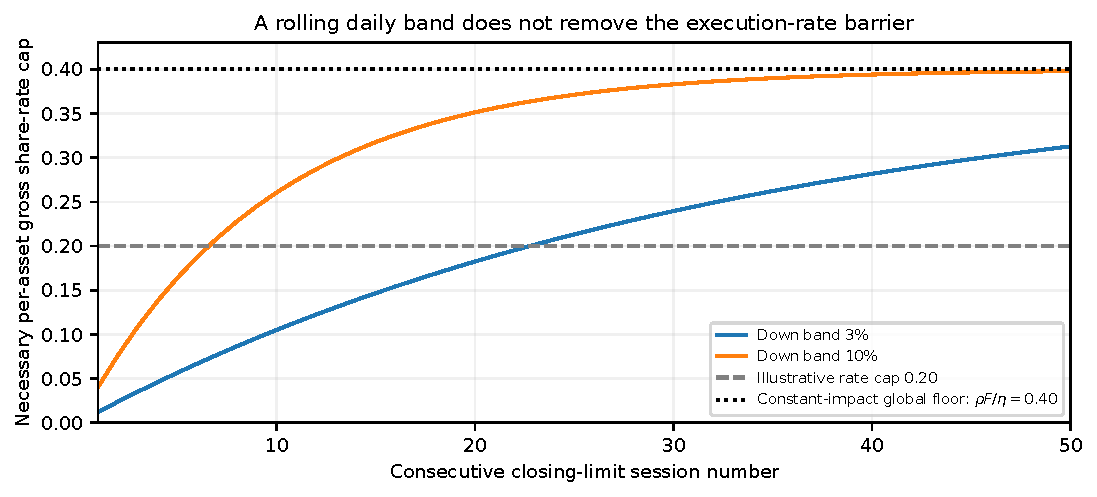
\includegraphics[width=.88\linewidth]{../../supplementary/figures/multiday_rate_frontier.pdf}
\caption{\textbf{反复跌停收盘的必要毛成交股数速率下限。} 主文的标量恒定冲击必要速率公式，用于标量恒定冲击比较模型，$F=\eta=1$、$\rho=0.4$、$\tau=20$。这些是逐资产\emph{必要}速率；成对执行、可用库存及补偿资产自身每日区间可能使实际市场阈值更高。}\label{fig:streak-rate}
\end{figure}
\begin{figure}[tbp]\centering
 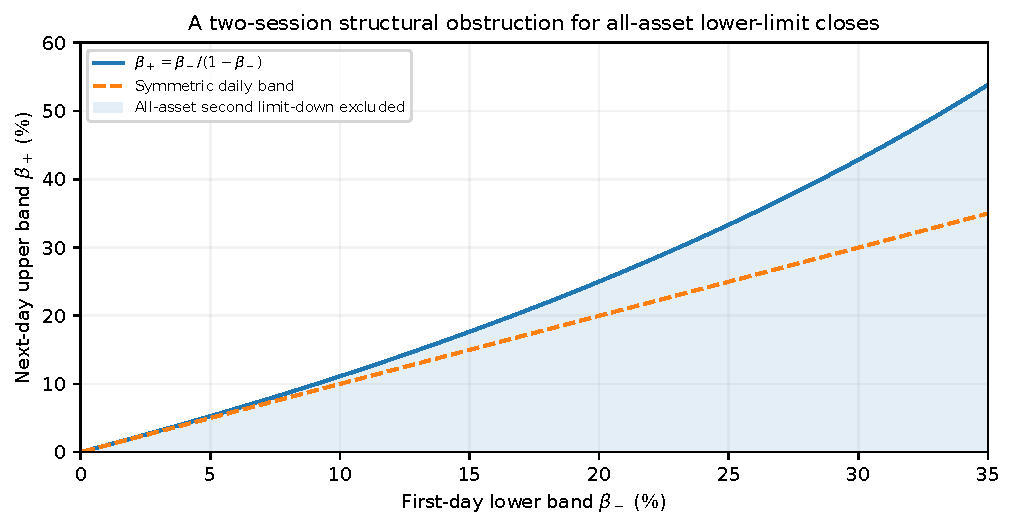
\includegraphics[width=.73\linewidth]{../../supplementary/figures/multiday_fullbreadth_obstruction.pdf}
\caption{\textbf{排除第二次全资产跌停收盘的参数区域。} 曲线下方区域满足 $(1+\beta_+)(1-\beta_-)\le1$。对称比例区间严格位于该区域内部。这是条件不变区域结果，而非全交易所订单队列模型。}\label{fig:streak-full-obstruction}
\end{figure}
\begin{figure}[tbp]\centering
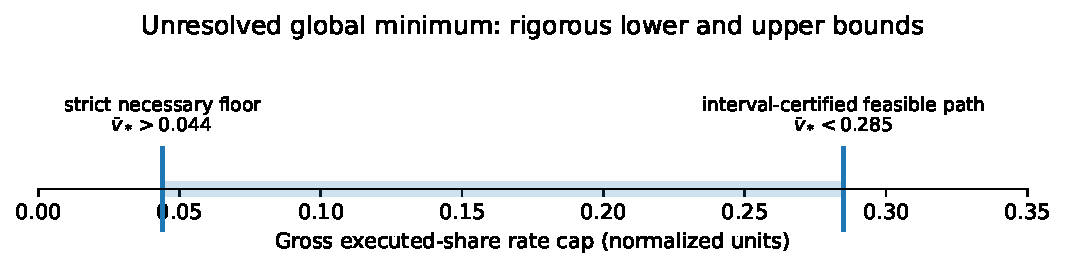
\includegraphics[width=.80\linewidth]{../../supplementary/figures/v7_minimum_rate_bracket.pdf}
\caption{\textbf{哪些量得到优化，哪些没有。} 现有系统性二次界的严格速率下限与经认证可行执行路径，共同夹住未知全局最小值 $\bar v_*$。该区间是逻辑上的容许性括界，而非统计置信区间。}\label{fig:v7bracket}
\end{figure}
\begin{figure}[tbp]\centering
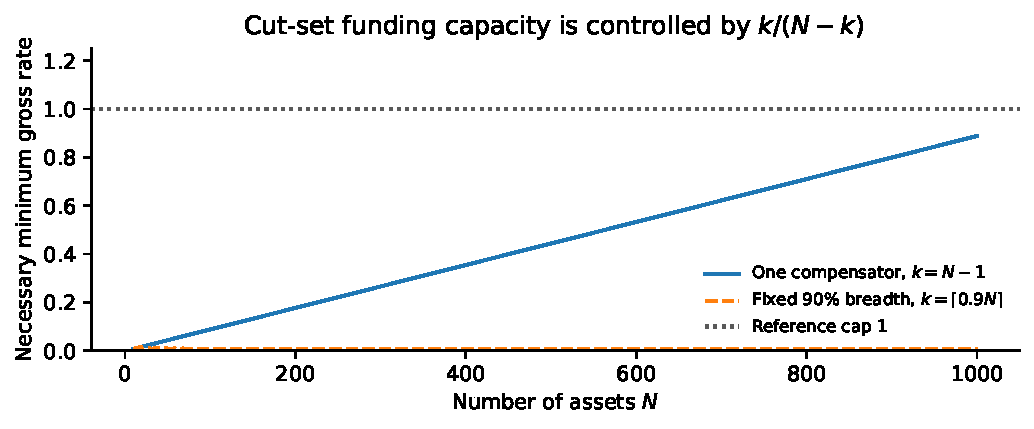
\includegraphics[width=.80\linewidth]{../../supplementary/figures/v7_cut_capacity_N.pdf}
\caption{\textbf{随下跌多数扩大而增长的资金容量约束。} 当单一资产吸收不断扩大的多数资产所产生的净配对美元时，主文中的必要第二日速率按 $k/(N-k)$ 增长。这并不证明对每个图示 $N$ 都存在可行市场。}\label{fig:v7cutN}
\end{figure}
\begin{figure}[tbp]\centering
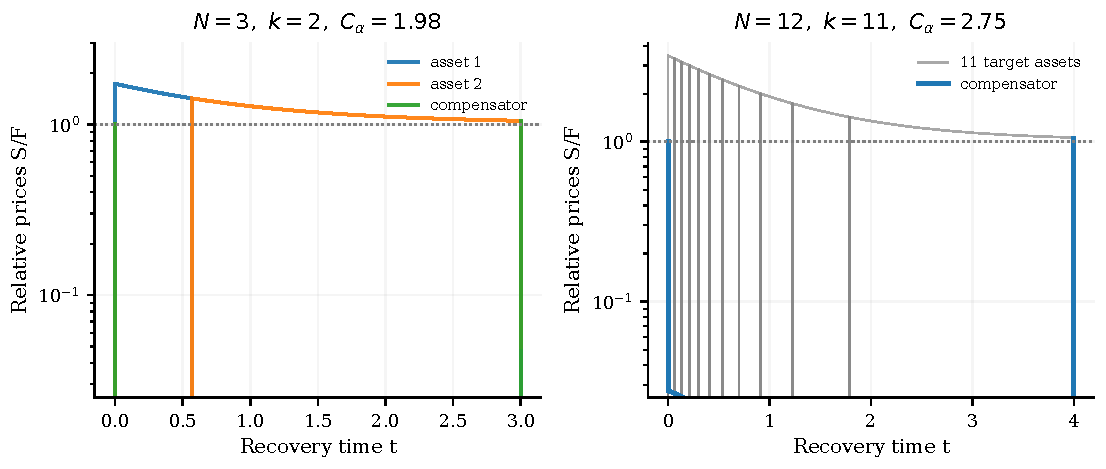
\includegraphics[width=.98\linewidth]{../../supplementary/figures/closed_flow_price_paths.pdf}
\caption{\textbf{终点净成交金额闭合的构造价格路径。} 对于 $N=3$ 及 $N=12$，一项补偿资产终价高于初值，其余 $N-1$ 项价格则产生共同目标对数损失 $L=3$。对数纵轴使接近零的价格仍可见。折点和跳跃是获准控制脉冲，而非模拟交易所事件。}\label{fig:paths}
\end{figure}
\begin{figure}[tbp]\centering
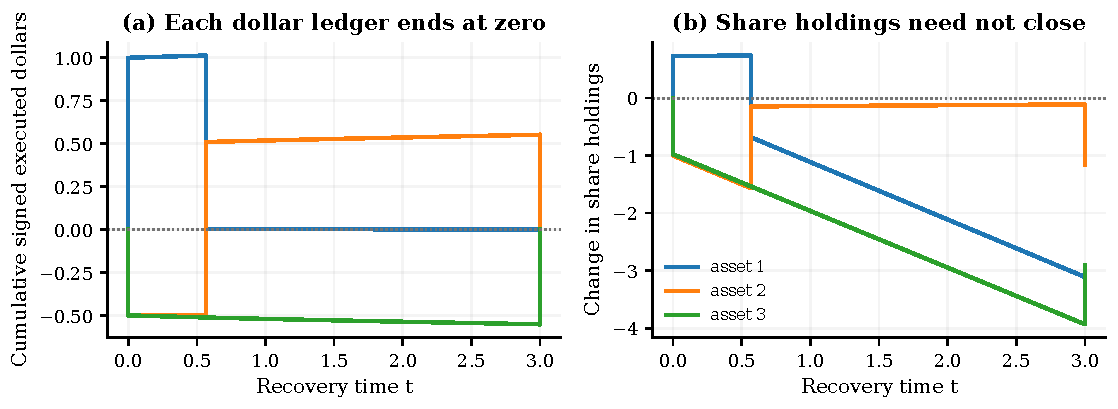
\includegraphics[width=.97\linewidth]{../../supplementary/figures/dollar_vs_share_closure.pdf}
\caption{\textbf{净成交美元不等于净股数。} 另一个 $N=3$、$k=2$、$T=3$、$L=5$ 见证对每项资产满足 $X_i(T)=0$（左），但净股数头寸通常不为零（右）。初始股数库存必须覆盖总卖出；仅有交易闭合并不能提供库存。}\label{fig:closure}
\end{figure}
\begin{figure}[tbp]\centering
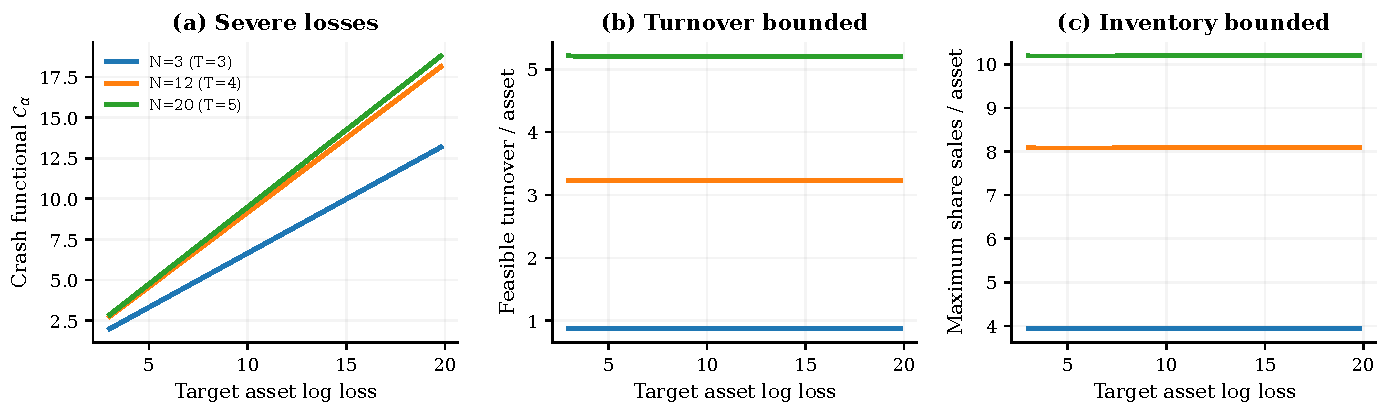
\includegraphics[width=.99\linewidth]{../../supplementary/figures/finite_resources_severe_crashes.pdf}
\caption{\textbf{在有界\emph{可行}资源下不断增加的危机严重程度。} 所选 $N=3,12,20$ 构造族分别采用 $k=N-1$ 及期限 $T=3,4,5$。终端目标价格对数损失增加时，达到的 $\mathcal C_\alpha$ 上升（左），而特定路径的逐资产换手（中）及最大累计股数卖出（右）保持有界。不同期限和价格是模型选择，并非跨市场校准或最优值。}\label{fig:finite}
\end{figure}
\begin{figure}[tbp]\centering
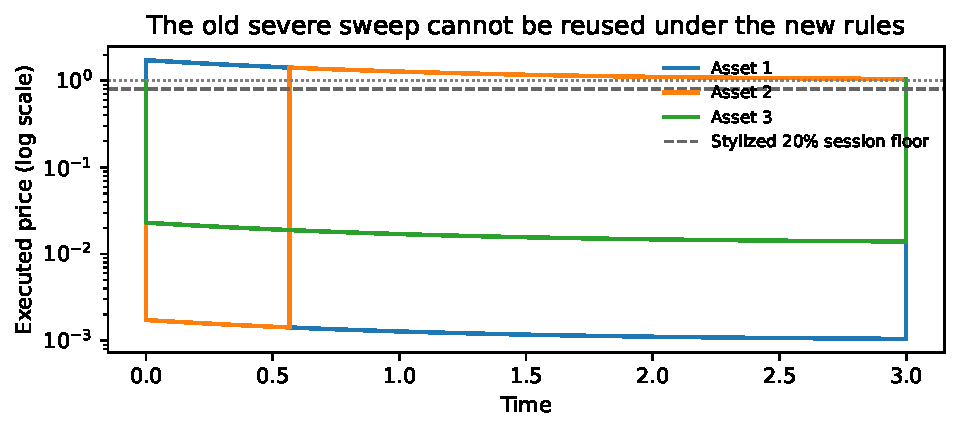
\includegraphics[width=.75\linewidth]{../../supplementary/figures/old_pulse_path_fails_limits.pdf}
\caption{\textbf{新执行限制下对旧严重损失路径的诊断性否决。} 不受限模型中的 $N=3$、$p=0$ 严重美元闭合见证越过简化的单时段 20\% 下限，并含有非零瞬时脉冲。因此，其精确闭合美元账簿\emph{不能}认证有限毛成交速率或价格限制协议下的可达性。}\label{fig:oldrejected}
\end{figure}
\end{document}
